% !TeX root = ../thuthesis-example.tex

\chapter{基础知识}
本章主要介绍本文所涉及的基础理论知识,首先概述了骨髓血细胞不同类别与发育阶段形态学特征。
然后介绍了骨髓血细胞图像数字化与数据集的构建。接着本文介绍了神经网络相关概念,最后对骨髓血细胞检测与识别软件系统涉及到的相关框架进行了介绍。
\section{骨髓血细胞图像及预处理}
\subsection{骨髓血细胞形态学介绍}
人体血细胞主要由骨髓内的造血干细胞分化而成。造血干细胞由髓系干细胞与淋系干细胞构成。其中髓系干细胞分化为粒细胞系统、红细包系统、单核细胞系统与巨核细胞系统,
淋系干细胞分化为浆细胞系统与淋巴细胞系统。不同系统的细胞按照发育成熟过程可以分为原始、早幼与成熟这三个阶段。粒细胞与红细胞的幼稚阶段可再具体划分为早幼,中幼与晚幼这
三个发育阶段。粒细胞系统根据细胞质内特殊颗粒对酸碱性物质亲和性,可分为嗜酸性粒细胞,嗜碱性粒细胞和中性粒细胞。骨髓血细胞六大系统血细胞的发育过程如图~\ref{fig:development}所示:
\begin{figure}
  \centering
  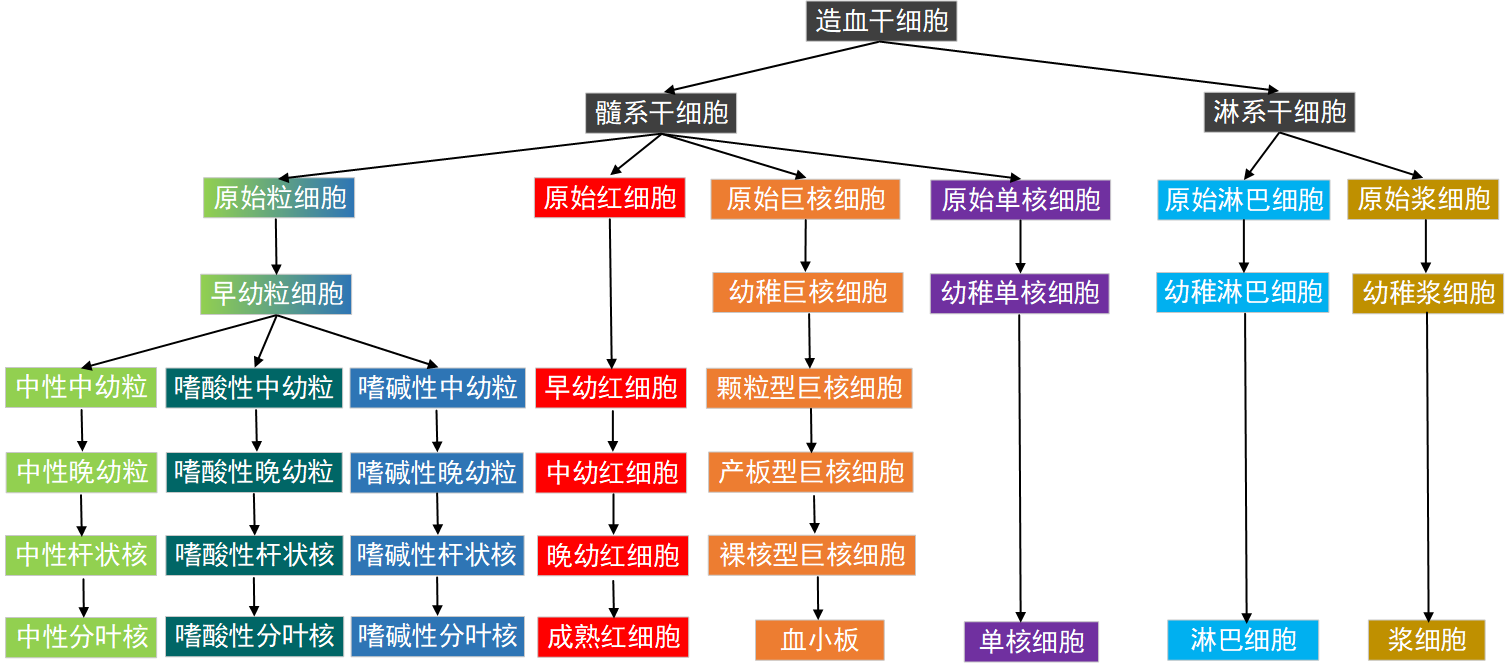
\includegraphics[width=1.0\linewidth]{development.png}
  \caption{骨髓血细胞发育成熟过程示意图}
  \label{fig:development}
\end{figure}

% \begin{itemize}
%   \item 原始细胞:胞体类圆形,直径在10\textasciitilde20微米。细胞核居中,呈圆形,染色质为粗细颗粒状,具有多个小而清晰的核仁。细胞质较少,无颗粒,呈蓝色或深蓝色。
%   \item 单核细胞:胞体呈现圆形或椭圆形,直径在14\textasciitilde25微米。细胞核扭曲折叠,常位于胞体中央或一侧,染色质疏松,核仁消失。细胞质通常为浅灰蓝色,可见空泡与紫红色的粉尘样颗粒。
%   \item 淋巴细胞:胞体为类圆形或不规则,直径在12\textasciitilde15微米。细胞核染色质致密,呈现索块状,形态上存在凹陷或者切迹。细胞质极少,呈现淡蓝色无颗粒。
%   \item 浆细胞:胞体常呈椭圆形或不规则,直径在12\textasciitilde16微米。细胞核多偏位,染色质聚集。细胞质为不透明的深蓝色,在细胞核周有淡染色带。
%   \item 有核红细胞:胞体规则类圆形,直径在7\textasciitilde10微米。细胞核为圆形位于细胞中央,内部含多个紫黑色团块。细胞质较多,无颗粒,为淡红色。
%   \item 早幼粒细胞:胞体较大,圆形或椭圆形,直径在12\textasciitilde25微米。细胞核较大,内部染色质细致,有清晰可见的核仁。细胞质为深蓝色,含有分布不均、形态不一的非特异性颗粒。
%   \item 中性中幼粒细胞:胞体为类圆形,直径在10\textasciitilde20微米。细胞核为半圆形或微凹陷,无核仁,染色质密集索块状。细胞质呈淡蓝色,其中存在大小均一,密集的淡粉红色中性颗粒。
%   \item 中性晚幼粒细胞:胞体类圆形,直径在10\textasciitilde16微米。细胞核呈半月形,存在凹陷,凹陷程度小于直径的1/2。染色质聚集小块状。细胞质多,淡蓝色,存在较多中性颗粒。
%   \item 中性杆状核细胞:胞体类圆形,直径10\textasciitilde15微米。细胞核为杆状、S形、U形等,凹陷程度大于直径的1/2,染色质粗块状。细胞质丰富,淡蓝色,充满中性颗粒。
%   \item 中性分页核细胞:胞体类圆形,直径10\textasciitilde14微米。细胞核通常分为2-5叶,之间通过核丝连接。细胞质丰富含有较多中性颗粒。
%   \item 嗜酸性粒细胞:胞体直径15\textasciitilde20微米。特点类似中性粒细胞,细胞质中存在大小分布均一,橘红色的嗜酸性颗粒。
% \end{itemize}
不同类别的骨髓血细胞胞体形状各异且细胞核与细胞浆会呈现出不同的颜色与纹理特征。表~\ref{table:cell_feature}
对本文主要关注的骨髓血细胞类别进行细胞核、细胞质等形态学方面的简要介绍。
\begin{longtable}{ccccc}
  % \centering
  \caption[Short Caption]{骨髓血细胞形态学特征}
  \label{table:cell_feature} \\
  % 下面是表头
  \hline
  \textbf{细胞名称} & \textbf{图像示例} & \textbf{胞体特征} & \textbf{细胞核} & \textbf{细胞质} \\ 
  \hline 
  \endfirsthead
  % 下面数字3的意思是表格的列数
  \multicolumn{5}{c}%
  {{\tablename\ \thetable{} --接上表}} \\
  \hline 
  \textbf{细胞名称} & \textbf{图像示例} & \textbf{胞体特征} & \textbf{细胞核} & \textbf{细胞质} \\ 
  \hline  
  % 注意这里把表头复制了一遍,因为在新的页面也会展示一下表头,不然表格不方便阅读
  \endhead
  \hline 
  % \multicolumn{5}{r}{{骨髓血细胞形态学特征}} \\ \hline
  \endfoot
  \endlastfoot
  原始细胞 & 
  \multicolumn{1}{m{0.15\textwidth}}{
  \begin{minipage}[b]{0.15\textwidth}
      \centering
      {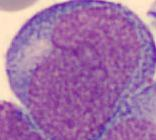
\includegraphics[width=0.9\textwidth]{cell_example/原始细胞.jpg}}
  \end{minipage}} &  
  \multicolumn{1}{m{0.15\textwidth}}{类圆形,直径10\textasciitilde20微米} & 
  \multicolumn{1}{m{0.20\textwidth}}{居中,呈圆形,染色质为颗粒状,具有多个小而清晰的核仁} & 
  \multicolumn{1}{m{0.20\textwidth}}{细胞质较少,无颗粒,呈蓝色或深蓝色}\\
  \midrule[0.5pt]
  单核细胞 & 
  \multicolumn{1}{m{0.15\textwidth}}{
  \begin{minipage}[b]{0.15\textwidth}
      \centering
      {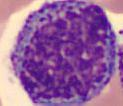
\includegraphics[width=0.9\textwidth]{cell_example/单核细胞.jpg}}
  \end{minipage}} &  
  \multicolumn{1}{m{0.15\textwidth}}{圆形或椭圆形,直径在14\textasciitilde25微米} & 
  \multicolumn{1}{m{0.20\textwidth}}{扭曲折叠,常位于胞体中央或一侧,染色质疏松,核仁消失} & 
  \multicolumn{1}{m{0.20\textwidth}}{通常为浅灰蓝色,可见空泡与紫红色的粉尘样颗粒}\\
  \midrule[0.5pt]
  淋巴细胞 & 
  \multicolumn{1}{m{0.15\textwidth}}{
  \begin{minipage}[b]{0.15\textwidth}
      \centering
      {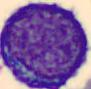
\includegraphics[width=0.9\textwidth]{cell_example/淋巴细胞.jpg}}
  \end{minipage}} &  
  \multicolumn{1}{m{0.15\textwidth}}{类圆形或不规则,直径在12\textasciitilde15微米} & 
  \multicolumn{1}{m{0.20\textwidth}}{染色质致密,呈现索块状,形态上存在凹陷或者切迹} & 
  \multicolumn{1}{m{0.20\textwidth}}{细胞质极少,呈现淡蓝色,无颗粒。}\\
  \midrule[0.5pt]
  浆细胞 & 
  \multicolumn{1}{m{0.15\textwidth}}{
  \begin{minipage}[b]{0.15\textwidth}
      \centering
      {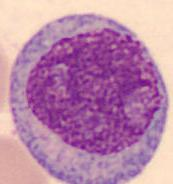
\includegraphics[width=0.9\textwidth]{cell_example/浆细胞.jpg}}
  \end{minipage}} &  
  \multicolumn{1}{m{0.15\textwidth}}{椭圆形或不规则,直径在12\textasciitilde16微米} & 
  \multicolumn{1}{m{0.20\textwidth}}{多偏位,染色质聚集} & 
  \multicolumn{1}{m{0.20\textwidth}}{细胞质为不透明的深蓝色,在细胞核周有淡染色带}\\
  \midrule[0.5pt]
  有核红细胞 & 
  \multicolumn{1}{m{0.15\textwidth}}{
  \begin{minipage}[b]{0.15\textwidth}
      \centering
      {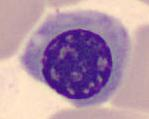
\includegraphics[width=0.9\textwidth]{cell_example/红细胞.jpg}}
  \end{minipage}} &  
  \multicolumn{1}{m{0.15\textwidth}}{规则类圆形,直径在7\textasciitilde10微米} & 
  \multicolumn{1}{m{0.20\textwidth}}{圆形位于细胞中央,内部含多个紫黑色团块} & 
  \multicolumn{1}{m{0.20\textwidth}}{细胞质较多,无颗粒,为淡红色。}\\
  \midrule[0.5pt]
  早幼粒细胞 & 
  \multicolumn{1}{m{0.15\textwidth}}{
  \begin{minipage}[b]{0.15\textwidth}
      \centering
      {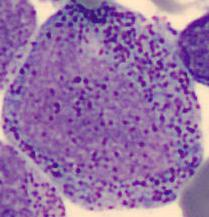
\includegraphics[width=0.9\textwidth]{cell_example/早幼粒细胞.jpg}}
  \end{minipage}} &  
  \multicolumn{1}{m{0.15\textwidth}}{较大,圆形或椭圆形,直径在12\textasciitilde25微米} & 
  \multicolumn{1}{m{0.20\textwidth}}{核较大,内部染色质细致,有清晰可见的核仁} & 
  \multicolumn{1}{m{0.20\textwidth}}{细胞质为深蓝色,含有分布不均、形态不一的非特异性颗粒}\\
  \midrule[0.5pt]
  中性中幼粒细胞 & 
  \multicolumn{1}{m{0.15\textwidth}}{
  \begin{minipage}[b]{0.15\textwidth}
      \centering
      {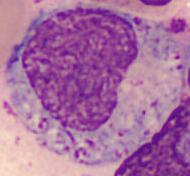
\includegraphics[width=0.9\textwidth]{cell_example/中幼粒细胞.jpg}}
  \end{minipage}} &  
  \multicolumn{1}{m{0.15\textwidth}}{类圆形,直径在10\textasciitilde20微米} & 
  \multicolumn{1}{m{0.20\textwidth}}{半圆形或微凹陷,无核仁,染色质密集索块状} & 
  \multicolumn{1}{m{0.20\textwidth}}{细胞质呈淡蓝色,其中存在大小均一,密集的淡粉红色中性颗粒}\\
  \midrule[0.5pt]
  中性晚幼粒细胞 & 
  \multicolumn{1}{m{0.15\textwidth}}{
  \begin{minipage}[b]{0.15\textwidth}
      \centering
      {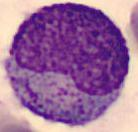
\includegraphics[width=0.9\textwidth]{cell_example/中性晚幼粒.jpg}}
  \end{minipage}} &  
  \multicolumn{1}{m{0.15\textwidth}}{胞体类圆形,直径在10\textasciitilde16微米} & 
  \multicolumn{1}{m{0.20\textwidth}}{呈半月形,存在凹陷,凹陷程度小于直径的1/2,染色质聚集小块状} & 
  \multicolumn{1}{m{0.20\textwidth}}{细胞质多,淡蓝色,存在较多中性颗粒}\\
  \midrule[0.5pt]
  中性晚幼粒细胞 & 
  \multicolumn{1}{m{0.15\textwidth}}{
  \begin{minipage}[b]{0.15\textwidth}
      \centering
      {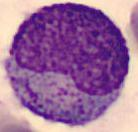
\includegraphics[width=0.9\textwidth]{cell_example/中性晚幼粒.jpg}}
  \end{minipage}} &  
  \multicolumn{1}{m{0.15\textwidth}}{胞体类圆形,直径在10\textasciitilde16微米} & 
  \multicolumn{1}{m{0.20\textwidth}}{呈半月形,存在凹陷,凹陷程度小于直径的1/2,染色质聚集小块状} & 
  \multicolumn{1}{m{0.20\textwidth}}{细胞质多,淡蓝色,存在较多中性颗粒}\\
  \midrule[0.5pt]
  中性杆状核细胞 & 
  \multicolumn{1}{m{0.15\textwidth}}{
  \begin{minipage}[b]{0.15\textwidth}
      \centering
      {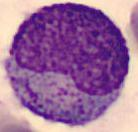
\includegraphics[width=0.9\textwidth]{cell_example/中性晚幼粒.jpg}}
  \end{minipage}} &  
  \multicolumn{1}{m{0.15\textwidth}}{胞体类圆形,直径在10\textasciitilde16微米} & 
  \multicolumn{1}{m{0.20\textwidth}}{呈半月形,存在凹陷,凹陷程度小于直径的1/2,染色质聚集小块状} & 
  \multicolumn{1}{m{0.20\textwidth}}{细胞质多,淡蓝色,存在较多中性颗粒}\\
  \midrule[0.5pt]
  中性分页核细胞 & 
  \multicolumn{1}{m{0.15\textwidth}}{
  \begin{minipage}[b]{0.15\textwidth}
      \centering
      {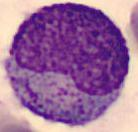
\includegraphics[width=0.9\textwidth]{cell_example/中性晚幼粒.jpg}}
  \end{minipage}} &  
  \multicolumn{1}{m{0.15\textwidth}}{胞体类圆形,直径在10\textasciitilde16微米} & 
  \multicolumn{1}{m{0.20\textwidth}}{呈半月形,存在凹陷,凹陷程度小于直径的1/2,染色质聚集小块状} & 
  \multicolumn{1}{m{0.20\textwidth}}{细胞质多,淡蓝色,存在较多中性颗粒}\\
  \midrule[0.5pt]
  嗜酸性粒细胞 & 
  \multicolumn{1}{m{0.15\textwidth}}{
  \begin{minipage}[b]{0.15\textwidth}
      \centering
      {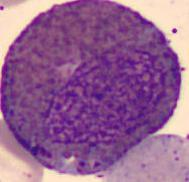
\includegraphics[width=0.9\textwidth]{cell_example/嗜酸性.jpg}}
  \end{minipage}} &  
  \multicolumn{1}{m{0.15\textwidth}}{直径15\textasciitilde20微米。} & 
  \multicolumn{1}{m{0.20\textwidth}}{类似中性粒细胞,染色质聚集索块} & 
  \multicolumn{1}{m{0.20\textwidth}}{大小分布均一,橘红色的嗜酸性颗粒}\\
  \midrule[0.5pt]
  嗜碱性粒细胞 & 
  \multicolumn{1}{m{0.15\textwidth}}{
  \begin{minipage}[b]{0.15\textwidth}
      \centering
      {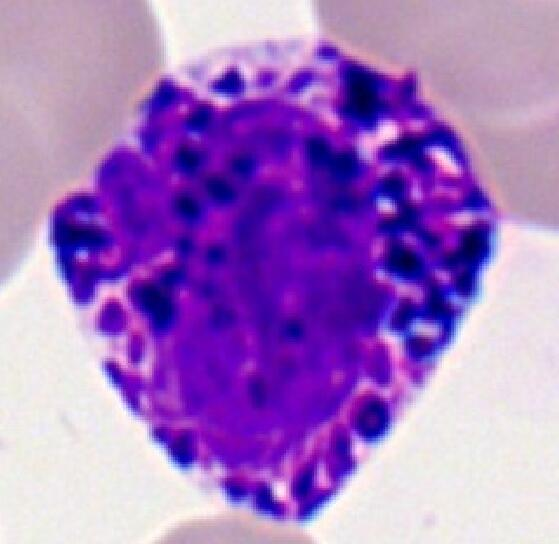
\includegraphics[width=0.9\textwidth]{cell_example/嗜碱性.jpg}}
  \end{minipage}} &  
  \multicolumn{1}{m{0.15\textwidth}}{直径10\textasciitilde15微米。} & 
  \multicolumn{1}{m{0.20\textwidth}}{染色质细致} & 
  \multicolumn{1}{m{0.20\textwidth}}{颗粒粗大,大小形态不一深紫红色的颗粒,部分颗粒覆盖在细胞核上}\\
  \bottomrule[1.5pt]
  \end{longtable}
\subsection{骨髓血细胞数据集与预处理}

\textbf{1)骨髓血细胞切片与数字化}

骨髓血细胞形态学检验技术是临床诊断血液疾病的重要依据。该过程由取材、制片、固定、染色、洗涤干燥与镜检等流程组成。首先通过骨髓穿刺采集骨髓液样本。接着将骨髓液
置于载玻片上制作成薄厚均一的涂片。在涂片制作完成后,使用甲醛或乙醇溶液将其固定。然后采用瑞特-吉姆萨染色剂进行适当时间的着色,染色完成后使用清水冲洗,待自然风干后以备观察。
最后使用光学显微镜对骨髓涂片进行观察,统计骨髓中不同类型血细胞的数量、比例,形态以及是否存在异常细胞,进行骨髓评估判断病情。具体如图~\ref{fig:cell_pre}所示:

\begin{figure}[htbp]
	\centering
	\begin{subfigure}{0.325\linewidth}
		\centering
		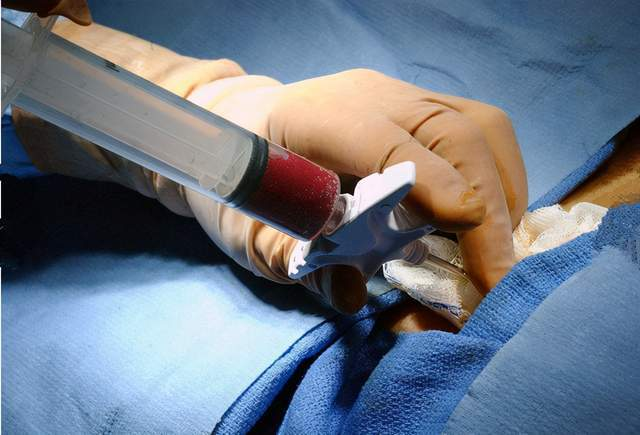
\includegraphics[width=0.95\linewidth, height=0.7\linewidth]{cell_pre/step1.jpg}
    \caption{}
	\end{subfigure}
	\centering
	\begin{subfigure}{0.325\linewidth}
		\centering
		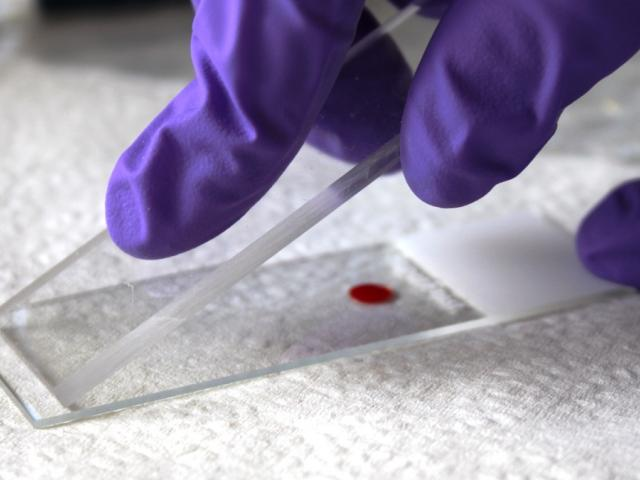
\includegraphics[width=0.95\linewidth, height=0.7\linewidth]{cell_pre/step2.jpg}
    \caption{}
	\end{subfigure}
	\centering
	\begin{subfigure}{0.325\linewidth}
		\centering
		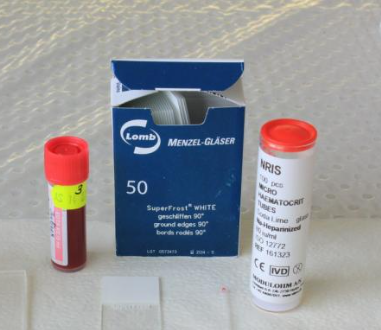
\includegraphics[width=0.95\linewidth, height=0.7\linewidth]{cell_pre/step3.jpg}
    \caption{}
	\end{subfigure}

	\centering
	\begin{subfigure}{0.325\linewidth}
		\centering
		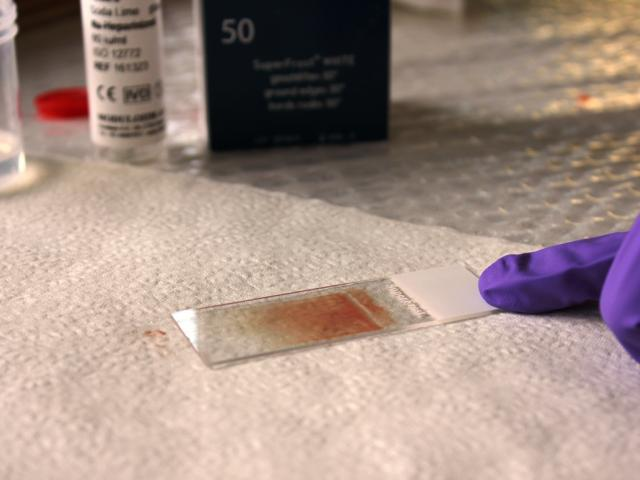
\includegraphics[width=0.95\linewidth, height=0.7\linewidth]{cell_pre/step4.jpg}
    \caption{}
	\end{subfigure}
	\centering
	\begin{subfigure}{0.325\linewidth}
		\centering
		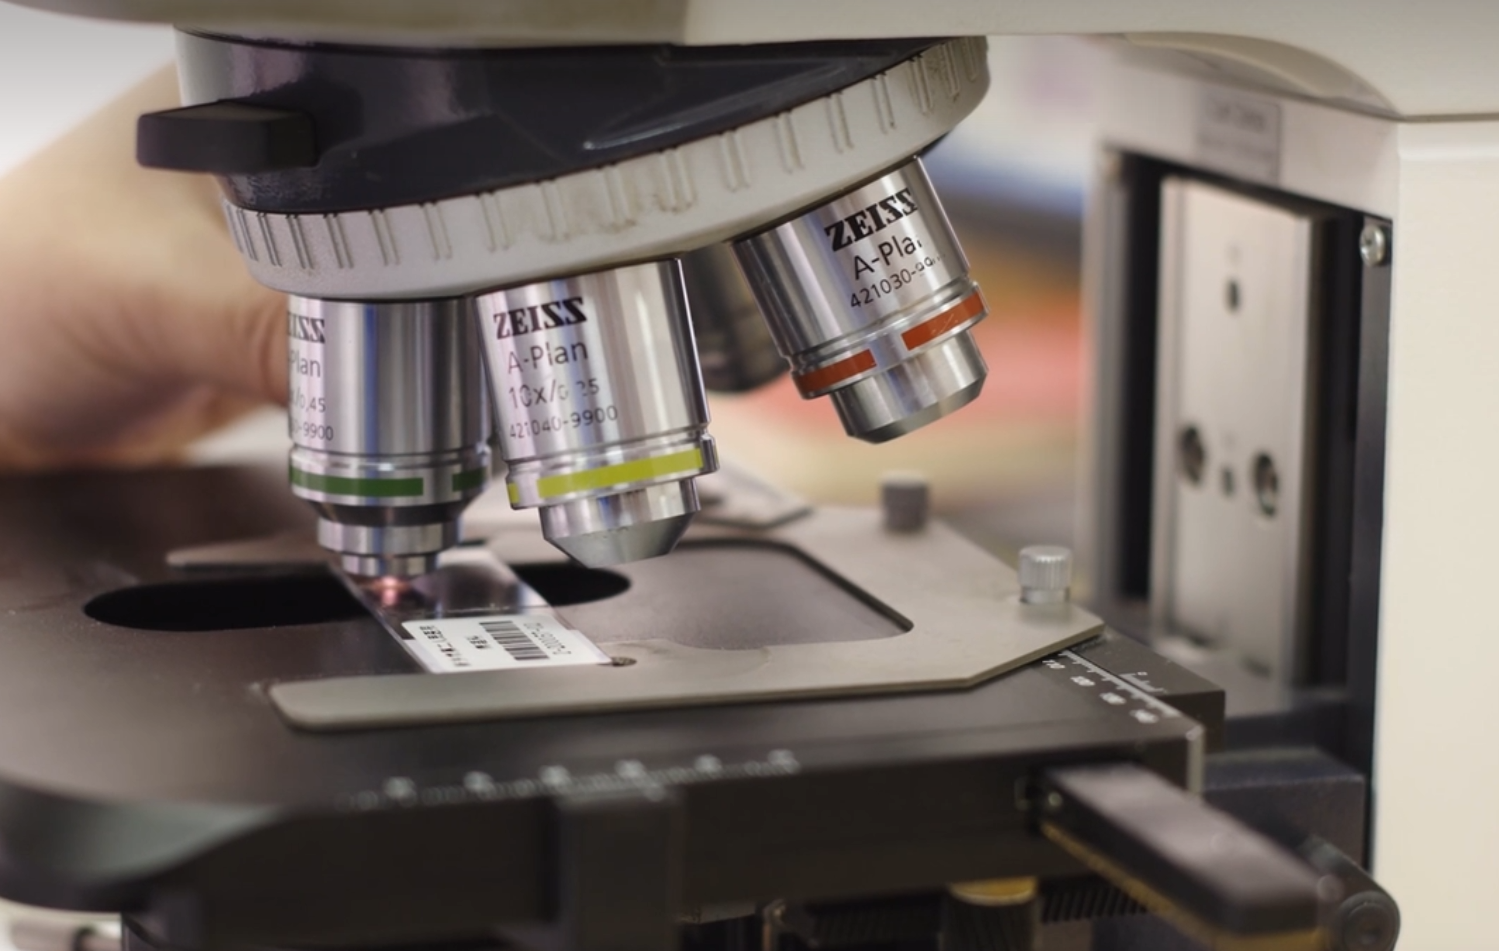
\includegraphics[width=0.95\linewidth, height=0.7\linewidth]{cell_pre/step5.jpg}
    \caption{}
	\end{subfigure}
	\centering
	\begin{subfigure}{0.325\linewidth}
		\centering
		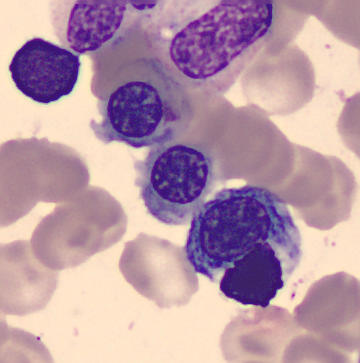
\includegraphics[width=0.95\linewidth, height=0.7\linewidth]{cell_pre/step6.jpg}
    \caption{}
	\end{subfigure}
	\caption{骨髓血细胞检验技术流程:(a)骨髓穿刺抽取骨髓液,(b)制备骨髓涂片,(c)瑞特-吉姆萨染色,(d)清洗晾干,(e)人工镜检判读,(f)骨髓形态学图片}
	\label{fig:cell_pre}
\end{figure}

对骨髓血细胞切片图像进行自动化评估分析首先需要对切片图像进行数字化,从而可以在计算机上进行存储,传输与分析。数字化技术可以为医学研究提供大量数据源,
促进医学研究与临床实验,方便医生进行更加快速与精准的病情分析。病理图像数字化技术由以下几个步骤组成。1)数字扫描:对制备好的组织切片使用数字成像与扫描设备生成数字图像,
一般通过CCD相机采用对焦深度法自动获取对焦位置并扫描成像。2)数字化处理:对图像进行去噪、分割与边缘检测等进一步提升图像质量。3)云存储与管理,将数字化图像存储在
云端服务器中,保证数据的完整性与安全。4)数字分析与诊断,利用计算机视觉等深度学习图像分析技术,对数字化后的病理图像进行分析与诊断,提高病理诊断的效率与准确性。

\textbf{2)数据集标注}

本文使用数据来源于实践基地邃蓝智能科技有限公司合作医院提供的脱敏数据。
数据标注是深度学习模型训练的基础,并且直接影响模型的性能和泛化能力。我们在合作医院病理医师的协作下对血细胞的边界框与类别信息进行精准的标注,完成了骨髓血细胞数据集(BMCD, Bone Marrow Cell Dataset)的制作。
原始数据集总共包含9250张骨髓血细胞图像,我们只关注图像中的有核细胞,而将成熟红细胞作为背景。因为缺少相关专业知识,我们仅标记出血细胞边界框的位置。
我们使用labelme软件作为标注工具,如图~\ref{fig:annotations}所示,针对每一张图像生成json标注文件,记录血细胞边界框的左上角与右下角的坐标,最后再将标注转化为coco格式,并将数据集划分为训练集、测试集与验证集。
经过检测网络,我们得到了单一血细胞图像,即图像中仅有一个完整的骨髓血细胞,这些图像再由经验丰富的病理医生完成类别标签的标注。

\begin{figure}
  \centering
  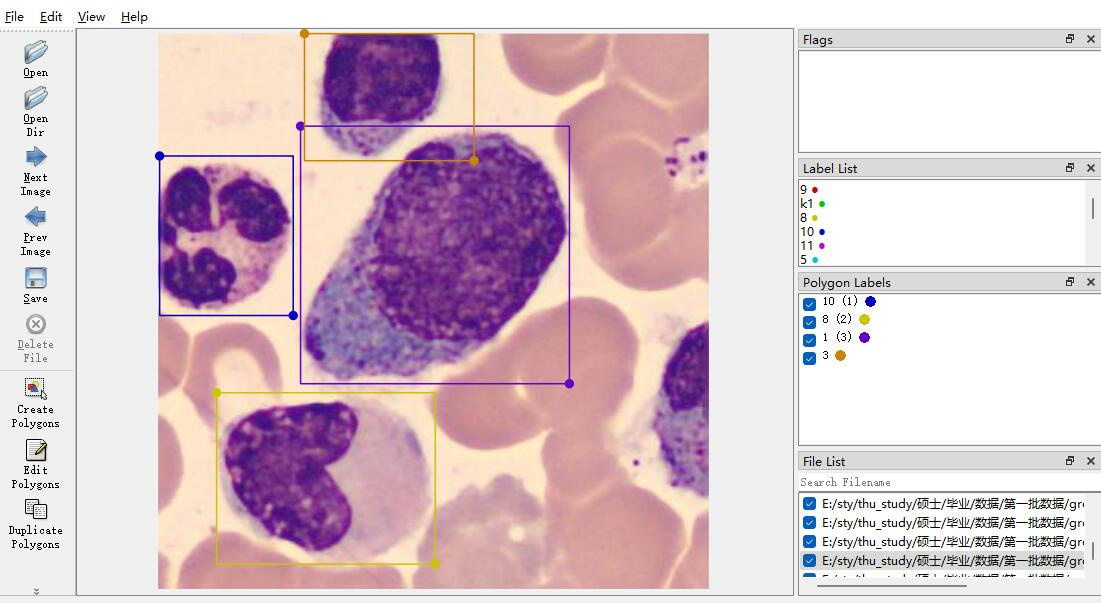
\includegraphics[width=0.8\linewidth]{annotations.jpg}
  \caption{labelme标注软件工具}
  \label{fig:annotations}
\end{figure}

大量的数据标注需要消耗很高的人力物力成本,我们采用主动学习技术去发掘数据集中高信息量的样本,提高标注的效率与精度,降低标注成本。
主动学习的基本思想是标注少量部分数据,利用已标注的数据训练深度学习模型。然后使用模型对未标注的数据进行预测,根据最大化熵、不确定度采样等进行排序,
筛选出不确定性最高的一些数据优先进行标注。不断迭代上述过程,直到标注与模型性能达到预期。具体而言,对于血细胞检测任务,首先标注将部分图像,然后训练Faster-RCNN网络
得到一个初步的检测模型,然后对每张图像进行检测,并生成标注json文件,再反馈到labelme标注软件中进行微调。针对血细胞识别任务,经过检测网络,我们得到了多张单个血细胞图像,首先完成部分
类别标注,训练初步的识别网络。对未标注的血细胞筛选出熵最大的预测样本反馈给病理医生进行核对。主动学习流程如图~\ref{fig:active}所示:

\begin{figure}
  \centering
  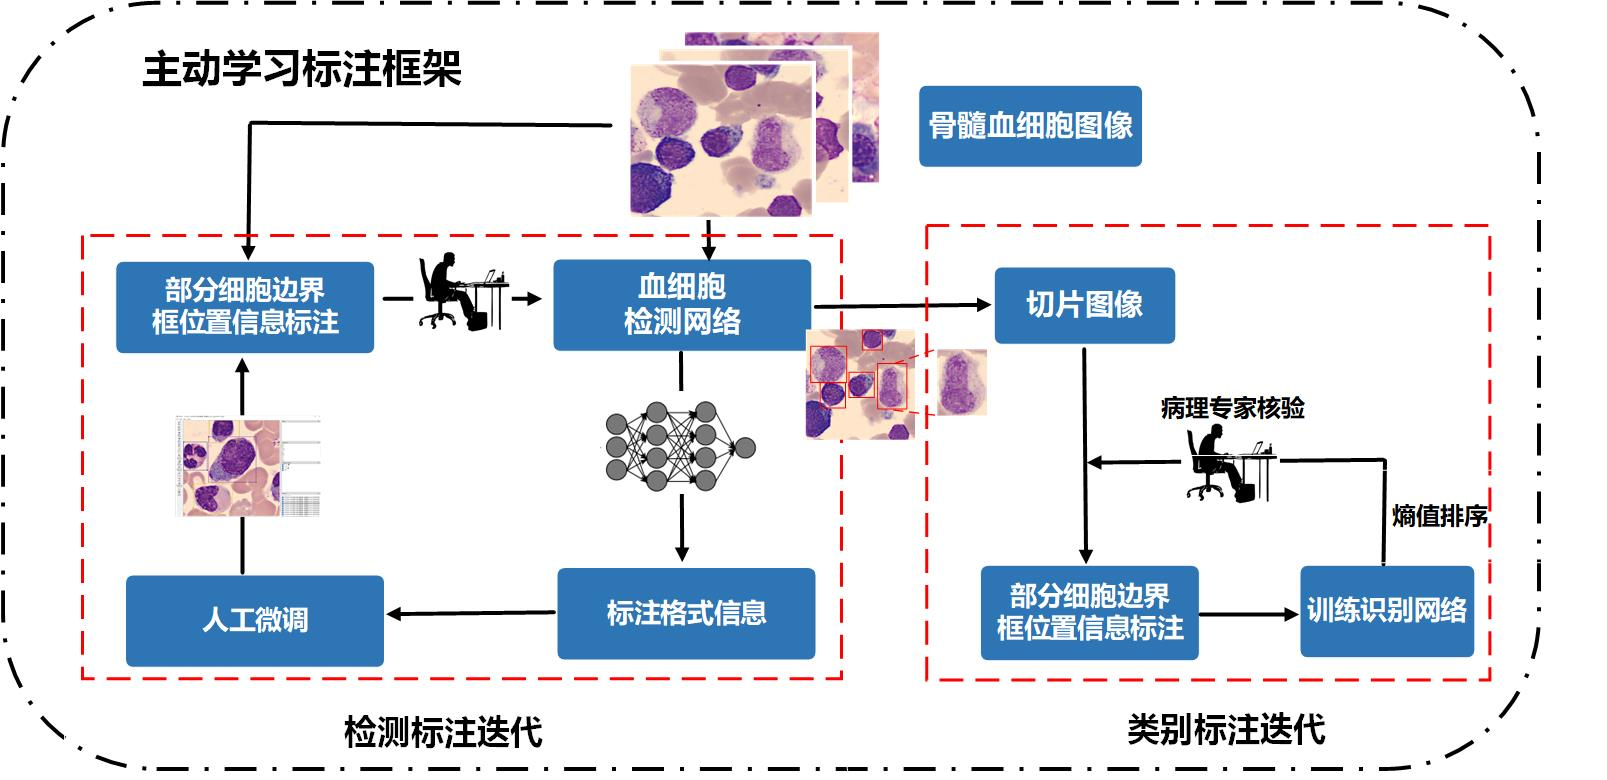
\includegraphics[width=1.0\linewidth]{active.jpg}
  \caption{主动学习标注框架示意图}
  \label{fig:active}
\end{figure}
\textbf{3)数据增强}

我们主要关注的五大系统细胞在人体内占比不同,粒细胞系统约占全部细胞的50\%,而浆细胞系统一般占比小于1.5\%,由于细胞天然就存在比例不均衡问题,其也导致了我们的数据集
存在严重的类别不平衡问题。例如单核细胞数量仅为有核红细胞数量的1/9。数据的不平衡会导致网络过多的关注数量较多的类别特征信息,数量较少类别易出现准确率与召回率的不均衡,影响模型的泛化性能。
为解决上述问题,本文对于数量较多的类别采用随机欠采样减少样本数量。对于数量较少的类别,采用翻转、旋转、添加噪声与色彩调整增加数据多样性。下面对数据增强方法进行简要介绍:
1)翻转:将图像沿水平或垂直方向进行镜像对称,生成新的图像。当图像$I(x,y)$沿水平方向进行翻转后,水平翻转图像为$I’(x, y)=I(w-x-1,y)$,其中w为原始图像宽度。
2)旋转:将图像沿着某个点或轴进行旋转,当图像$I(x,y)$以$(c_x, c_y)$为旋转中心时,旋转角度为$\theta$, 旋转后的图像为$I’(x, y)=I((x - c_x)\cos\theta - (y - c_y)\sin\theta + c_x, (x - c_x)\sin\theta - (y - c_y)\cos\theta + c_y)$。
3)添加噪声:常用的图像噪声包括高斯噪声、椒盐噪声与泊松噪声。高斯噪声是一种连续随机噪声,服从零均值、标准差为$\sigma$的正态分布,会使得图像变模糊。
椒盐噪声是离散随机噪声,图像中会出现亮点与暗点,降低图像的清晰度与对比。
4)色彩调整:常用方法包括了亮度调整、对比度调整、色相调整与饱和度调整。

\section{神经网络技术概述}
\subsection{神经元与梯度优化}

\textbf{1)神经元}

神经网络发展历史最早可以追溯到20世纪五十年代,当时研究人员受到神经科学启发,模拟生物神经元结构提出了神经网络。
神经元是神经网络的基本单元,其结构如图~\ref{fig:neuron}所示,由输入、加权、激活函数、输出这四个部分组成。
\begin{figure}
  \centering
  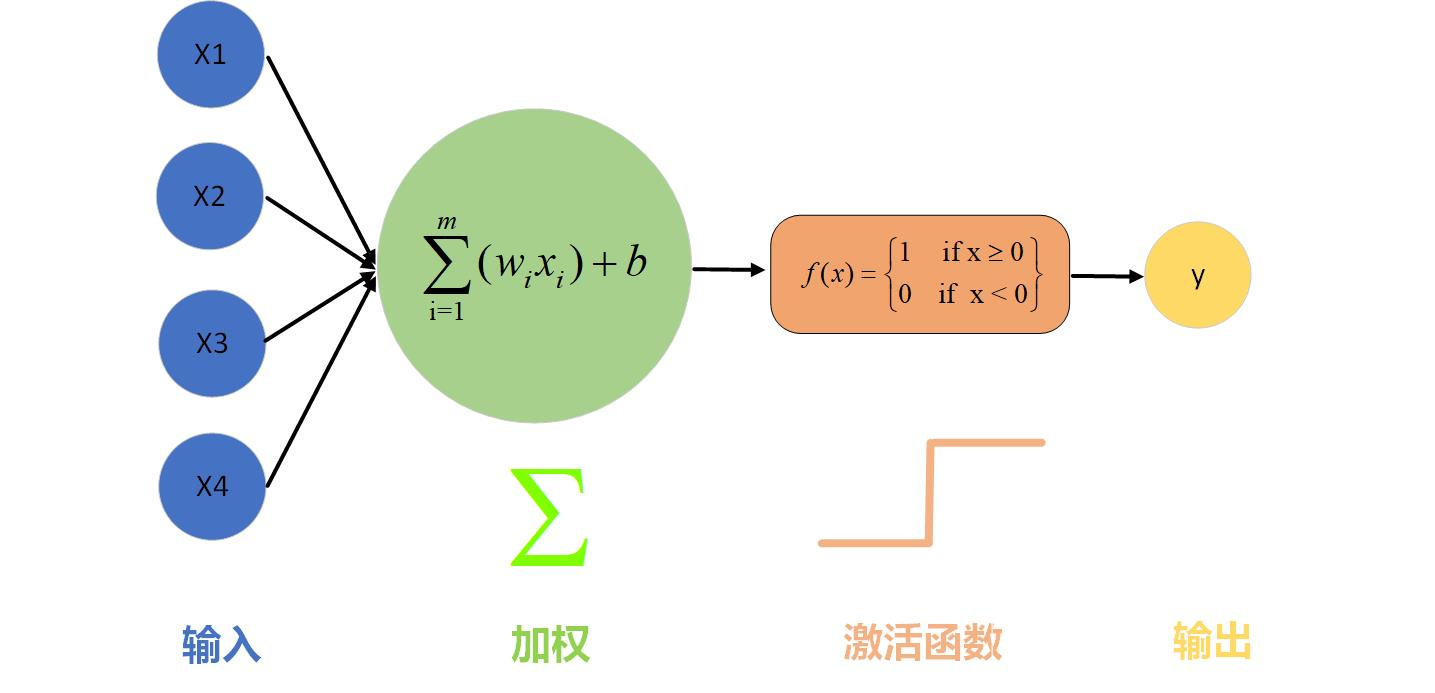
\includegraphics[width=0.8\linewidth]{neuron.jpg}
  \caption{神经元结构示意图}
  \label{fig:neuron}
\end{figure}

输入部分,神经元接收其他神经元的信息$x_1, x_2, \dots, x_4$,每个输入与权重进行关联。加权部分表示神经元对于输入部分的敏感程度。
激活函数将加权和进行变换,保证输出数值范围并引入非线性的特性。输出部分是激活函数处理后的结果,如式~\ref{eq:neuron}所示,可作为后续神经元的输入。
\begin{equation}
  h(x) = f({{\bf{W}}^T}{\bf{x}}) = f(\sum\limits_{i = 1}^m {{w_i}{x_i} + b})
  \label{eq:neuron}
\end{equation}

式~\ref{eq:neuron}中$f(\cdot)$为激活函数。常用的激活函数有修正线性单元函数(Rectified linear unit function,ReLU)、双曲正切函数、sigmoid函数等。

\textbf{2)感知机}

感知机由美国心理学家弗兰克·罗森布\cite{1958perceptron}在1958年提出,它是一种最简单的神经网络,拓扑结构如图~\ref{fig:perceptron}所示。
网络包含了输入层、隐含层与输出层,前一层的每个神经元都与后一层的神经元相连。前一层神经元输出信息传递到下一层神经元的过程称为前向传播。
该过程可以用一系列矩阵乘法与激活函数进行描述,若输入数据为$x$, 网络结构总共有$L$层,则前向传播过程可以表示为:
\begin{equation}
  \begin{aligned}
  z^{1} & =W^{1} x+b^{1} \\
  a^{1} & =g^{1}\left(z^{1}\right) \\
  & \vdots \\
  z^{L} & =W^{L} a^{L-1}+b^{L} \\
  a^{L} & =g^{L}\left(z^{L}\right)=\hat{y}
  \label{eq:perceptron}
\end{aligned}
\end{equation}

其中 $z^{l}$ 表示第$l$层的未激活值,$a^{l}$ 表示第$l$层的激活值,$W^{l}$ 和 $b^{l}$ 分别表示第$l$层的权重矩阵和偏置向量。
\begin{figure}
  \centering
  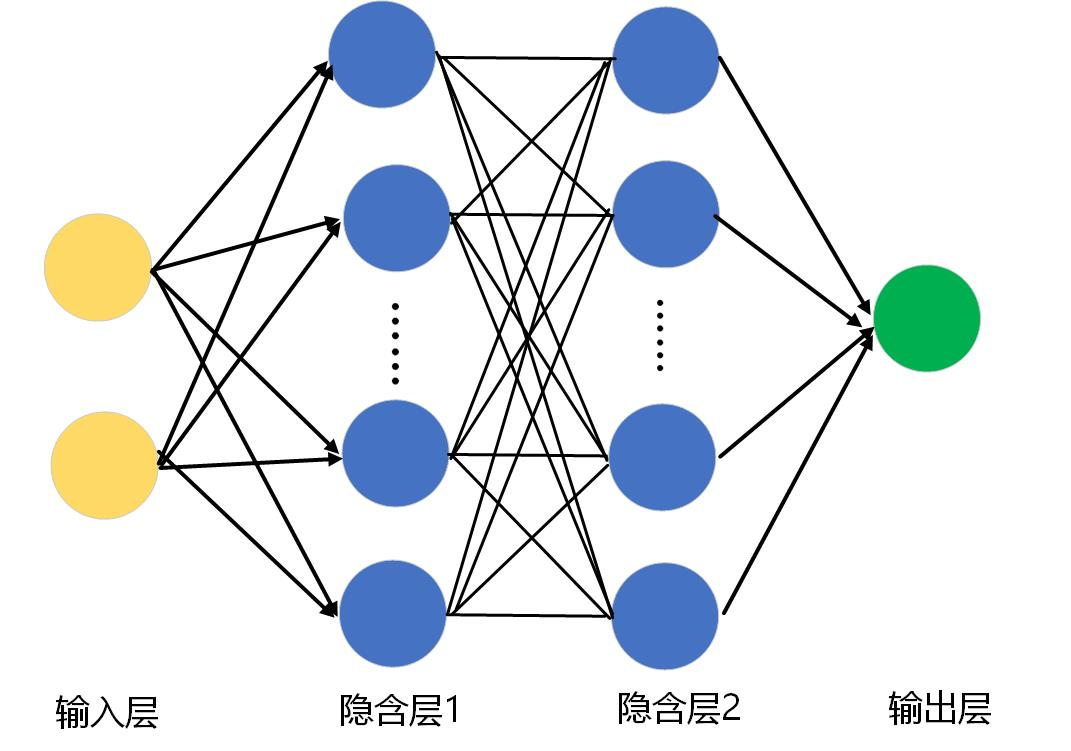
\includegraphics[width=0.65\linewidth]{perceptron.jpg}
  \caption{感知机网络模型示意图}
  \label{fig:perceptron}
\end{figure}

\textbf{3)反向传播与梯度优化}

反向传播全称是误差反向传播(back propagation,BP),是用于神经网络训练的算法。神经网络经过前向传播得到网络预测值,采用
损失函数衡量预测值与真实值之间的误差。通过损失函数最小化计算神经网络参数的导数,然后调整更新神经网络权重参数以减小误差。不断迭代上述过程,
直到模型参数收敛。

假设 $L$ 为损失函数,$w_{ij}^k$ 表示第$k$层第$i$个神经元到第$j$个神经元之间的权重,$a_j^l$ 表示$l$ 层的第$j$个神经元的非激活值
$z_j$ 表示第 $j$ 层神经元输出,$\sigma_l(\cdot)$为第l层激活函数。反向传播过程计算过程如下:
\begin{enumerate}[label=(\alph*)]
  \item 网络进行前向传播得到预测值
  \item 定义输出层的误差$\delta_k^L$为损失函数对输出层非激活值的导数,如式~\ref{eq:delta}所示,
  \begin{equation}
    \delta_k^L = \frac{\partial L}{\partial a_k^L} = \frac{\partial L}{\partial z_k^L} \frac{\partial z_k^L}{\partial a_k^L}
    \label{eq:delta}
  \end{equation}
  \item 对于中间隐含层,可以通过链式法则求出第$l$层的传播误差$\delta_j^l$
  \begin{equation}
    \begin{aligned}
    \delta_j^l & = \frac{\partial L}{\partial a_j^l} = \frac{\partial L}{\partial z_j^l} \frac{\partial z_j^l}{\partial a_j^l} \\
    \frac{{\partial L}}{{\partial z_j^l}} & = \sum\limits_i^{} {\frac{{\partial L}}{{\partial a_i^{l + 1}}}} \frac{{\partial a_i^{l + 1}}}{{\partial z_j^l}} = \sum\limits_i^{} {\delta _i^{l + 1}} w_{ij}^{l + 1} \\
    \delta_j^l & = \frac{{\partial L}}{{\partial a_j^l}} = \sigma _l^\prime \left( {a_j^l} \right)\sum\limits_i^{} {w_{ij}^{l + 1}} \delta _i^{l + 1}
    \end{aligned}
    \label{eq:delta_l}
  \end{equation}
  \item 计算损失函数对于某一隐含层$l$权重$w_{ij}^k$的梯度值
  \begin{equation}
    \frac{{\partial L}}{{\partial w_{ij}^l}} = \frac{{\partial L}}{{\partial a_j^l}}\frac{{\partial a_j^l}}{{\partial w_{ij}^l}} = \delta_j^l z_i^{l - 1}
    \label{eq:delta_w}
  \end{equation}
  \item 若训练的学习率为$\eta$,随机抽取小批量样本$\left\{ {\left( {{{\bf{x}}_m},{{\bf{y}}_m}} \right)} \right\}_{m = 1}^{{N_0}}$,权重值的更新如下
  \begin{equation}
    w_{ij}^{l(\tau  + 1)} = w_{ij}^{l(\tau )} - \eta \frac{1}{{{N_0}}}\sum\limits_{m = 1}^{{N_0}} {\frac{{\partial {L_m}}}{{\partial w_{ij}^l}}}
    \label{eq:update}
  \end{equation}
  \item 重复上述步骤,直到损失函数达到极小值,得到收敛后最优的网络模型参数
\end{enumerate}

\textbf{4)优化算法}

在定义好损失函数后,通过误差反向传播算法调整网络中的权重参数,使得网络在训练数据集上的误差最小化。但传统梯度优化算法面临着诸多困难,
损失函数存在着大量的鞍点与平坦区域,可能收敛到局部极小值点。此外训练集数据量巨大,计算全部数据梯度非常耗时。针对上述问题,研究学者提出了小批量
随机梯度下降算法(mini-batch stochastic gradient descent),每次从训练集中随机抽取出m个样本组成小批量样本,对于这组样本计算梯度均值用于更新权重系数,如式~\ref{eq:msgd}所示
\begin{equation}
  \begin{aligned}
    \boldsymbol{g}  & \leftarrow \nabla_{w}\left(\frac{1}{m} \sum_{i=1}^{m} L\left(f\left(\boldsymbol{x}_{i} ; \boldsymbol{w}\right), \boldsymbol{y}_{i}\right)\right) \\
    \boldsymbol{w}  & \leftarrow  \boldsymbol{w} - \eta \boldsymbol{g}
  \end{aligned}
  \label{eq:msgd}
\end{equation}

小批量随机梯度下降算法面临着学习率选择困难问题。学习率过小收敛慢,过大导致震荡。Adagrad是最早的自适应学习率优化算法。
其设置了一个梯度二阶累积统计量$r$,每次使用小批量梯度平方和来更新$r$,权重更新如下
\begin{equation}
  \begin{aligned}
    \boldsymbol{r}  & \leftarrow   \boldsymbol{r}  +  \boldsymbol{g}^2\\
    \boldsymbol{w}  & \leftarrow  \boldsymbol{w} - \frac{\eta}{\sqrt{r + \delta}} \boldsymbol{g}
  \end{aligned}
  \label{eq:adagrad}
\end{equation}

Adagrad算法在训练后期,由于累计平方很大,网络更新停止。针对上述问题,RMSProp优化算法设置了一个衰减系数$\rho$,r的更新公式如下:
\begin{equation}
  \begin{aligned}
    \boldsymbol{r}  & \leftarrow  \rho \boldsymbol{r}  + (1-\rho) \boldsymbol{g}^2\\
  \end{aligned}
  \label{eq:Rmsprop}
\end{equation}

Adam优化算法(Adaptive Moment estimation)集成了动量与多种优化算法的优势,使梯度更新更平滑,适用于大多数的神经网络优化问题,是目前应用最广泛的梯度优化算法。
该算法计算了梯度的一阶矩$\boldsymbol{m}$与二阶矩$\boldsymbol{v}$,一阶矩类似于动量,降低梯度随机变化大的影响,二阶矩用于控制自适应学习率。参数更新公式如下:
\begin{equation}
  \begin{aligned}
    \boldsymbol{m_t}  & \leftarrow  \beta_1 \boldsymbol{m_{t-1}}  + (1 - \beta_1) \boldsymbol{g_t} \\
    \boldsymbol{v_t}  & \leftarrow  \beta_2 \boldsymbol{v_{t-1}}  + (1 - \beta_2) \boldsymbol{g_t^2} \\
    \boldsymbol{\hat{m_t}} &  \leftarrow \frac{\boldsymbol{m_t}}{1 - \beta_1} \\
    \boldsymbol{\hat{v_t}} &  \leftarrow \frac{\boldsymbol{v_t}}{1 - \beta_2} \\
    \boldsymbol{w}  & \leftarrow  \boldsymbol{w} - \frac{\eta}{\sqrt{\boldsymbol{\hat{v_t}} + \delta}} \boldsymbol{\hat{m_t}}
  \end{aligned}
  \label{eq:Adam}
\end{equation}




\subsection{卷积神经网络}

\textbf{1)基本概念与结构}

卷积神经网络(Convolutional Neural Network, CNN)是计算机视觉领域应用最广泛的神经网络。相比于传统的全连接神经网络,
CNN引入了卷积层与池化层,通过稀疏连接与权值共享,可以更加有效的提取空间数据的特征模式,降低了模型参数量与计算复杂度。
卷积神经网络由多个卷积层、池化层、全连接层等组成,典型结构如图~\ref{fig:cnn}所示。

\begin{figure}
  \centering
  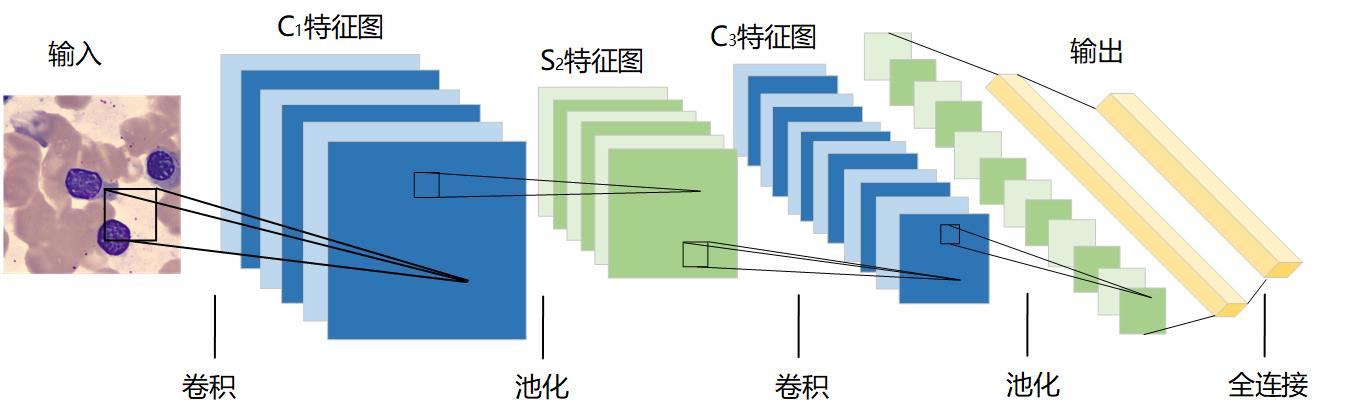
\includegraphics[width=1.0\linewidth]{cnn.jpg}
  \caption{典型卷积神经网络结构示意图}
  \label{fig:cnn}
\end{figure}

\textbf{2)卷积层}

卷积层是卷积神经网络的基础结构。卷积层由多个卷积核构成,每个卷积核用于抽取不同的图像特征,输出一个卷积通道特征。
如图\ref{fig:conv}所示,输入特征图有三个通道,该卷积层有四个卷积核,最终输出包含四个通道的特征图。
多个卷积通道拼接后组成卷积层的输出。卷积核将输入特征图局部区域像素与卷积核对应元素相乘后求和,再将结果写入到输出特征图对应位置,如式~\ref{eq:conv}所示。
卷积核有四个描述参数,卷积核大小(kernel size)、步幅(stride)、边界扩充(stride)、输入与输出通道数量(channel)。
通过卷积操作抽取图像特征,再不断将特征进行组合,形成最终图像的特征描述。
\begin{equation}
  \begin{array}{l}
    y(m, n)=\sum_{i} \sum_{j} I(i, j) h(m-i, n-j) \\
    =\sum \sum I(m-i, n-j) h(i, j)
    \end{array}
  \label{eq:conv}
\end{equation}

卷积核大小为卷积核的宽度与高度,通常小卷积核来提取边缘、线条等纹理特征,大卷积核提取高级抽象特征。步幅控制
卷积核在图像上滑动的距离,决定了输出特征图的大小。步幅增大使得特征图大小减小,从而降低网络的计算复杂度。
边界扩充是图像边界上进行零填充,可以使得图像边缘像素作为卷积核的中心进行卷积,避免边缘信息丢失。卷积核的输入通道数量由
输入特征图的通道数决定。输出通道数据量为卷积核的个数,提高卷积核数量可以增加提取特征的丰富性,从而比高网络的表达能力。

\begin{figure}
  \centering
  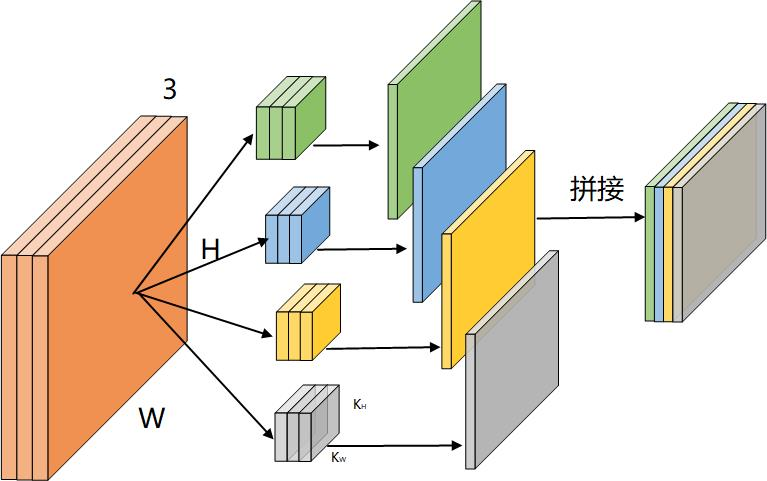
\includegraphics[width=0.7\linewidth]{conv.jpg}
  \caption{CNN卷积层示意图}
  \label{fig:conv}
\end{figure}

\textbf{3)池化层}

池化层位于卷积层后,池化也称为降采样,主要用于特征选择与降维,降低特征图大小,从而降低后续卷积等操作的计算量,
同时能够让网络学习图像有效特征,提高网络的铝棒性与泛化性,避免过拟合问题。
池化操作通过池化核来完成,池化核在图像局部区域内进行下采样,用一个值代表当前区域特性。然后根据步长在图像上从左向右,从上到下滑动。
常用的池化方式有最大池化与平均池化,最大池化在特征图局部区域中选择最大值来表征此区域,最大池化可以使得特征图对比更加显著。
平均池化在局部区域特征图中使用均值来表征此区域,整体特征信息更加平滑。
通常池化核大小选择为$2 \times 2$,然后将输入特征图划分为多个相同大小的区域,以最大池化的方式进行。

\begin{figure}
  \centering
  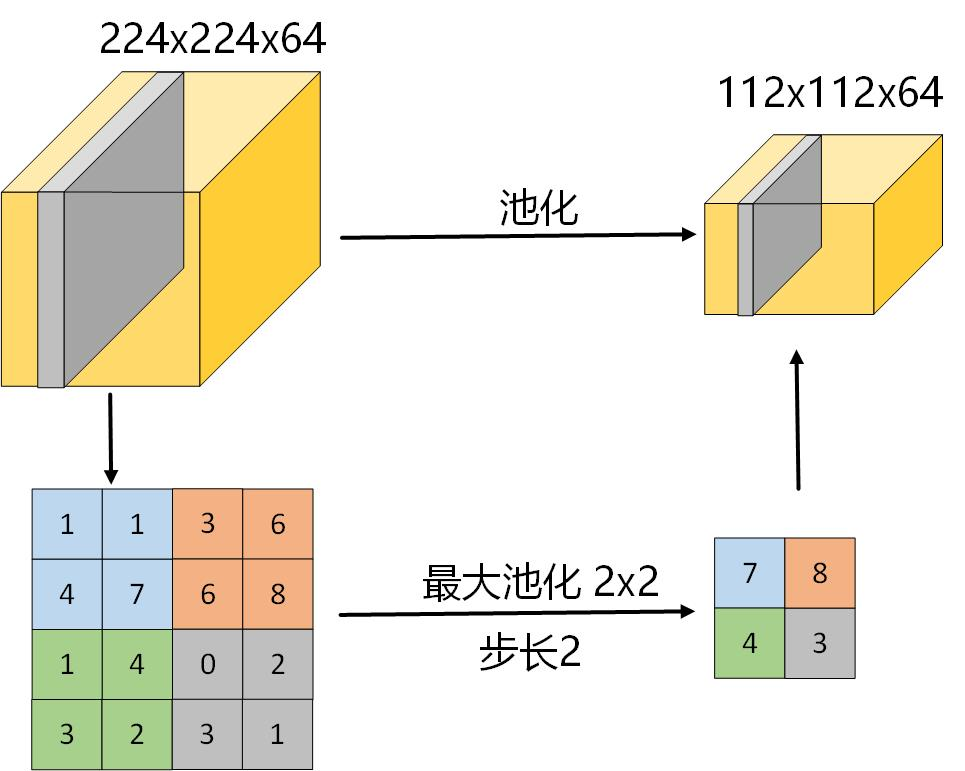
\includegraphics[width=0.6\linewidth]{pool.jpg}
  \caption{CNN池化层示意图}
  \label{fig:pool}
\end{figure}


\section{软件开发相关技术}
本节主要介绍骨髓血细胞检测与识别软件开发使用的技术框架。首先介绍前端核心技术,Vue框架与Element UI组件库。
然后介绍后端使用的框架Django与深度学习模型部署工具ONNX。

\subsection{前端技术}

前端技术主要用来构建优美的用户图像界面、并提供良好的用户交互。随着互联网技术的飞速发展,前端web技术已经步入到
2.0时代。无论是在移动端还是PC端,我们都能体验到设计精妙绝伦的界面,并进行丰富多元的交互,极大提升了用户的浏览
效率与用户体验。前端开发的三个核心基础要素是超文本标记语言HTML、层叠样式表与Javascript语言。目前,随着前端技术的不断
发展,已存在多种前端框架与组件库工具,可以帮助开发人员可以快速搭建出风格优美统一的界面,提升开发效率。本小结对软件开发
使用到的前端框架与组件库进行简要介绍:

\textbf{1)HTML、CSS与Javascript}

HTML的全称是超文本标记语言(Hypertext Markup Language),是用来构建和布局界面内容的描述语言。该语言使用标签结构与属性标记
对文字、图像、视频、超链接、表格等内容进行不同形式的呈现。目前HTML主要遵循HTML5规范,该版本引入了更多种类的标签、使得界面结构更加清晰。
此外引入了更多的新表单控件。支持多种音频、视频等多媒体形式,无需三方插件。在性能方面也使用了多线程通信与缓存技术,可以更加快速的访问资源
与处理请求。

CSS的全称是层叠样式表(Cascading Style Sheets),它是一种样式表语言,主要用来定义HTML元素的表现形式。通过CSS可以对于页面上的元素
进行精确的布局描述,并为元素添加圆角、阴影、动画或者复杂的过度效果。此外CSS可以根据设备屏幕大小与分辨率对页面的布局和样式进行响应以适应不同的设备。

Javascript是一种解释型的轻量级Web开发编程语言,作为编程代码嵌入到HTML页面后,可以由浏览器进行解释执行。通过javascript语言可以
实现动态效果与用户的交互,例如用户提交表单验证、响应用户的请求、动态界面等。
通过上述三种技术来构建内容,设计样式与行为控制,开发者可以快捷、高效、灵活的创建出更好用户图形界面应用。

\textbf{2)VUE前端框架}

随着前端功能越来越复杂,出现了多种前端框架来简化前端编程开发。JQuery是最早的前端框架,对javascript进行了多种封装,可以更加便捷的操作文档对象模型(Document Object Model)。
在JQuery的基础上演化出MVC架构,即模型(Model)-视图(View)-控制器(Controller)的架构。该架构将界面、数据业务逻辑、信息输入更新进行分离,
使得代码易于维护与升级。目前主流的前端架构是MVVM架构,如图~\ref{fig:mvvm}所示,MVVM是模型(Model)-视图(View)-视图模型(ViewModel)的缩写。模型代表
软件应用的数据模型与业务逻辑。视图是用户界面,将数据可视化呈现。ViewModel监听模型数据改变并控制视图行为,它通过数据的双向绑定将模型与视图连接起来,模型中的变化会
自动同步到视图中,视图中的变化也同步到模型中。Vue.js是一款轻量级、渐进式的MVVM前端框架。相比于其他框架拥有如下的优势:双向数据绑定,避免操作DOM,易于维护;
组件化,将界面拆分为多种组件,每个组件拥有自己的view与model,代码复用性与模型化程度更高;响应式设计,采用虚拟DOM与Diff算法优化渲染效率,极大减少了修改DOM元素的次数;
生态环境丰富,Vue有大量的插件,方便扩展,社区活跃,大量优秀的开发者在持续的对框架进行维护、更新与完善。

\begin{figure}
  \centering
  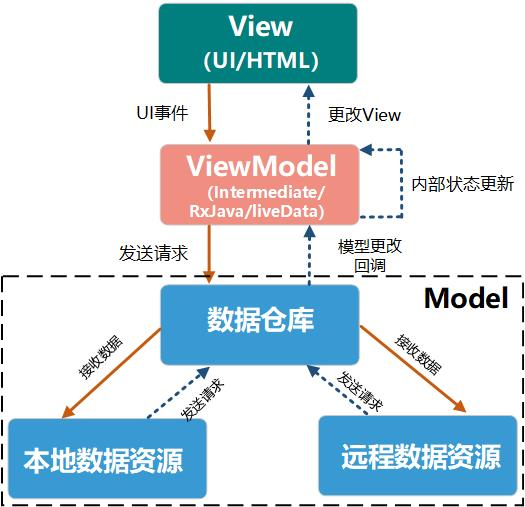
\includegraphics[width=0.7\linewidth]{MVVM.jpg}
  \caption{MVVM框架示意图}
  \label{fig:mvvm}
\end{figure}

\textbf{3)Element-UI组件库}

Element-UI是一套基于Vue 2.0的桌面端组件库,提供了一系列开箱即用的精美UI组件,如表单、布局、弹窗、导航、数据展示等多种组件。这些组件的设计简洁、优美、风格统一,可以帮助开发人员 
高效快速的构建美观、易用的界面程序。Element-UI提供的API接口简单易学,可以轻松的自定义组件扩展。该组件库使用了虚拟滚动技术,极大的提高了页面的渲染性能。

\subsection{后端技术}

\textbf{1)后端框架}

在计算机领域,框架是指一套规范、标准、结构完整的程序模版。框架通常包含了一系列的库、工具与接口,开发者可以按照框架的规范快速进行应用程序开发,
减少重复工作,提高开发效率同时保障软件的可靠性。目前各个编程语言均有自己的Web后端框架,这些框架各具特色,一些框架亮点在分布式、高性能,一些框架优势在与高成熟与高扩展度。

在诸多的编程语言中,Python是一种解释型、面向对象的高级程序设计语言。其优势在于拥有丰富的标准库、框架与详细的官方文档,并且可以方便的跨平台运行。
Python语言被广泛应用在多种领域如数据分析、人工智能、后端开发。在深度学习领域,Pytorch是由Facebook开发的基于Python的开源深度学习框架,在学术界与工业界广泛使用。
本文使用Pytorch框架进行模型训练。

Django是一个基于Python的开源Web后端框架。它最早由Adrian Holovaty和Simon Willison在2003年开发,用于维护劳伦斯集团旗下的
几个新闻网页。该框架于2005年7月在BSD许可证下发布,截至目前,Django已经经历过三个大版本的迭代。最新的Django 3.0版本于2019年12月发布,
主要引入了对异步通信编程的原生支持,可以支持更高并发、高流量的应用程序。Django框架基于MTV架构,MTV的全称是模型(Model)-模板(Template)-视图(View)。
模型是数据业务逻辑,主要进行数据库的增删改查。模板可以动态生成HTML,决定如何对内容进行展示。视图封装负责处理用户请求与返回响应的逻辑。框架结构如~\ref{fig:django}所示:
Django框架具有如下的优势,(1)高度可扩展,框架的每个组件均可以替换与修改,便于添加与修改功能。(2)强大数据库访问组件,可以根据Model快速更改数据库模式,便捷的进行数据迁移,
数据库操作代码简洁。(3)安全性,Django内置了多种安全机制和功能,包括了跨站请求伪造保护、跨站脚本攻击保护、SQL注入保护与认证与授权等。

\begin{figure}
  \centering
  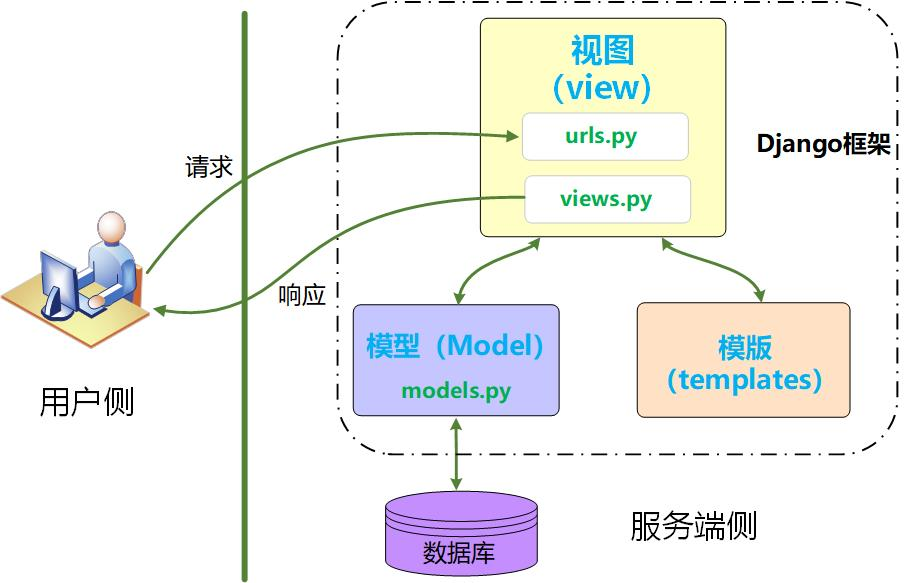
\includegraphics[width=0.75\linewidth]{django.jpg}
  \caption{Django框架示意图}
  \label{fig:django}
\end{figure}



\textbf{2)ONNX模型部署工具}

在深度学习模型训练结束后,我们要让模型能够在生产环境中运行。部署时首先要对运行环境进行配置,此外还要对网络结构进行优化精简提高模型的推理性能。
目前针对神经网络的部署主要采用深度学习框架-中间表示-推理引擎这种流水线方式。首先是定义模型结构并选择一种深度学习框架进行训练。之后,将模型结构与参数转化成一种通用的中间表示,
在此基础上进行效率优化。最后将中间表示文件在含有推理引擎的硬件平台上高效运行。

开放式神经网络交换(Open Neural Network Exchange,ONNX)是微软与Facebook在2017发布的用于描述计算图的一种格式。它是一种开放的规范,定义了模型的
标准数据类型,内置运算算子与可扩展的计算图模型。ONNX目前支持多种深度学习框架如Pytorch、Tensorflow、Caffe2、Mxnet等。在Pytorch中可以使用$torch.onnx.export()$函数将Pytorch模型
转为ONNX格式的静态计算图模型。ONNX Runtime是由微软开发的一个跨平台、高性能的机器学习推理引擎,它是ONNX文件的运行环境,在该环境下可以读取并运行.onnx 文件。
目前ONNX Runtime支持多种硬件环境,包括了CPU、GPU、地平线的BPU、华为海思等国产推理芯片。完成上述流程实现了深度学习算法的落地与部署
